\documentclass{article}
\usepackage[spanish]{babel}
\usepackage[utf8]{inputenc}
\usepackage{graphicx}
\usepackage{amsmath}
\usepackage{caption}
\usepackage[hidelinks]{hyperref}
\usepackage{geometry}
\usepackage{lmodern}
\usepackage{verbatim}
\usepackage{listings}
\lstset{basicstyle=\ttfamily\footnotesize, breaklines=true}
\geometry{margin=2.5cm}

\title{Percolation Project}
\author{Anaya Lizarazo, Bryan Johan; Pinilla Correa, Santiago \& Torres Otálora, Erick}
\date{\today}

\begin{document} 

\maketitle

\section{Introducción} 

La percolación es un fenómeno físico y matemático que describe el comportamiento colectivo de elementos conectados en una red, lo cual puede servir para simular el movimiento de fluidos en medios porosos. En este proyecto se estudia el modelo de percolación porosa por sitios sobre una red cuadrada bidimensional de tamaño \( L \times L \). Este modelo consiste en recorrer cada uno de los sitios de la matriz y ocuparlo con una probabilidad \( p \). A partir de esta ocupación aleatoria, se identifican los conglomerados de sitios vecinos ocupados, conocidos como \emph{clusters}.

Para el reconocimiento eficiente de estos clusters se implementó el algoritmo de Hoshen-Kopelman, que permite etiquetar de manera rápida y sin redundancias los distintos conglomerados conectados de la matriz. Con esta información es posible determinar si existe un cluster que conecta los bordes opuestos de la red, es decir, si el sistema \emph{percola}.

En la figura \ref{fig:lattice_clusters} se ilustran dos representaciones de una red: una antes de identificar los clusters en donde los sitios ocupados se representan con 1 y otra después de aplicar el algoritmo de Hoshen-Kopelman, donde cada cluster ha sido etiquetado y representado con un color diferente.

\begin{figure}[ht]
    \centering
    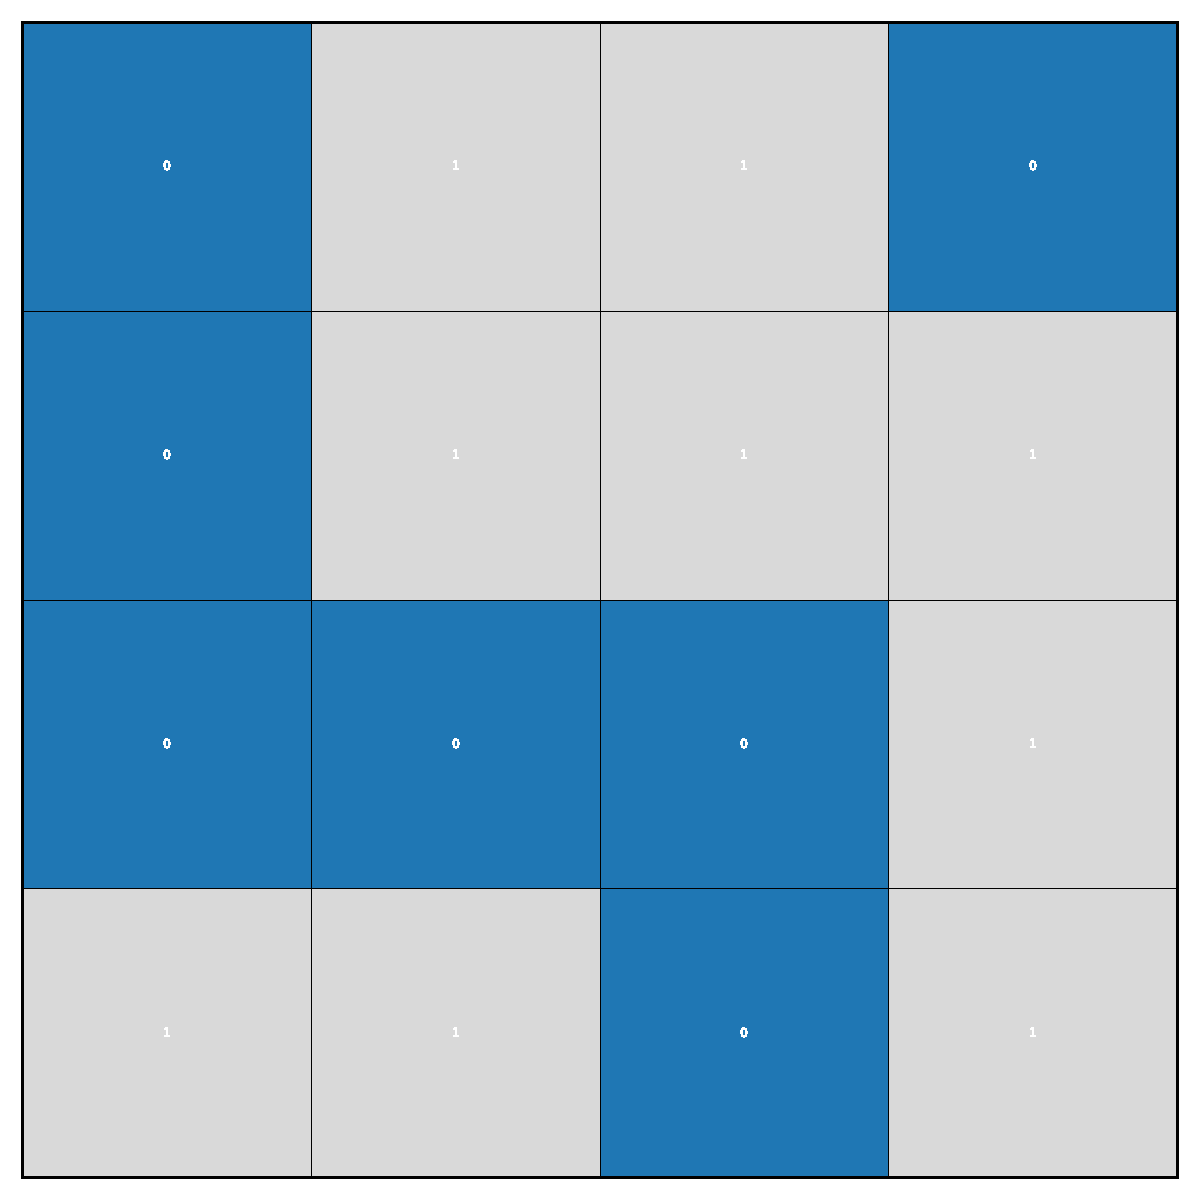
\includegraphics[width=0.45\textwidth]{figures/lattice.pdf}
    \hfill
    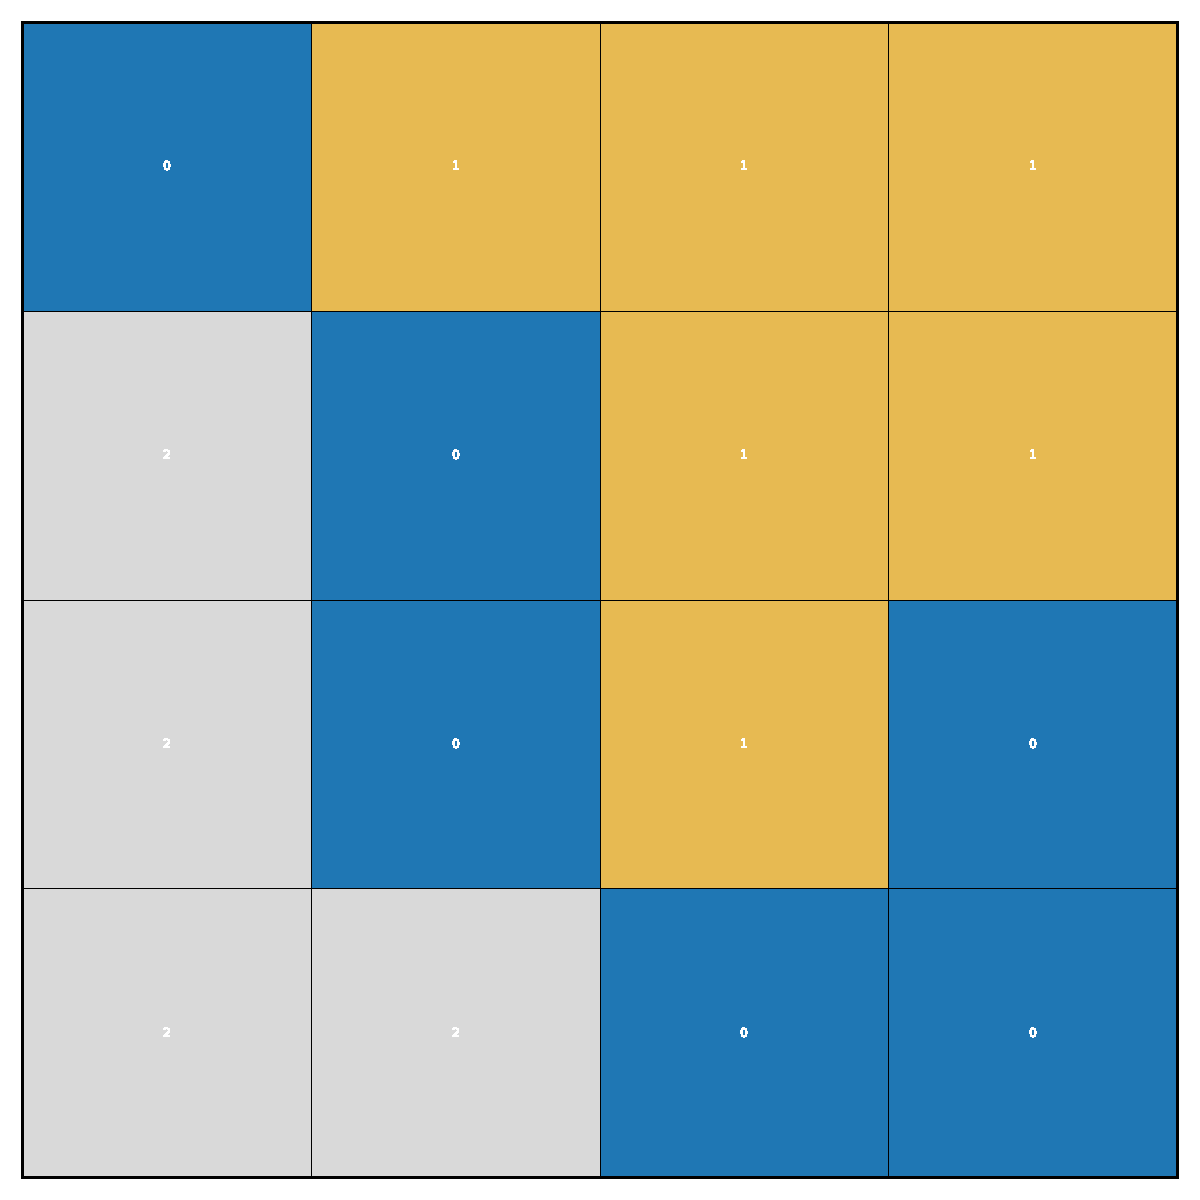
\includegraphics[width=0.45\textwidth]{figures/clusters.pdf}
    \caption{(Izquierda) Lattice de tamaño \( L \times L \) con ocupación aleatoria según probabilidad \( p \). (Derecha) Identificación de clusters mediante el algoritmo de Hoshen-Kopelman.}
    \label{fig:lattice_clusters}
\end{figure}
En el límite termodinámico (\(L \to \infty\)), se define una probabilidad crítica \(p_{c}\). Por debajo de este umbral (\(p < p_{c}\)), no existe clúster percolante de tamaño macroscópico, mientras que para \(p \ge p_{c}\) aparece con probabilidad uno un clúster de tamaño infinito que conecta la red.

El objetivo de este artículo es estudiar el comportamiento de la probabilidad de percolación y del tamaño del cluster percolante en función de los parámetros \(L\) y \(p\), con el fin de comprobar las predicciones teóricas de la teoría de percolación. Además, se analizará la eficiencia del código implementado para distintos niveles de optimización, empleando herramientas de profiling como \texttt{gprof} y \texttt{perf}, con el propósito de identificar posibles optimizaciones y mejorar el rendimiento computacional en la simulación de redes percolates.


\section{Resultados de Percolación}

A continuación se presentan los resultados numéricos obtenidos para la probabilidad de percolación y el tamaño promedio del clúster percolante más grande (normalizado con el tamaño del sistema \( L \times L \)) en función de la probabilidad de llenado \(p\) y para distintos tamaños de red \(L = 16,\,32,\,64,\,128,\,256,\,512\). Dado que se trata de una probabilidad y de un tamaño promedio, se ejecutó el programa 10 veces para poder realizar la estadística sobre estos resultados.

En la Figura \ref{fig:perc_prob} se muestra la probabilidad de percolación \(P(L,p)\) frente a \(p\). Cada curva corresponde a un tamaño \(L\) distinto. Se observa que, para valores bajos de \(p\), la probabilidad de que exista un clúster que conecte bordes opuestos es cero, mientras que al incrementarse \(p\) la probabilidad crece en el intervalo \(p\in(0.5, 0.6)\) para despues ser uno. Además, a medida que \(L\) aumenta, la transición se vuelve más pronunciada y la curva se desplaza hacia el valor crítico \(p_c \approx 0.6\). Este comportamiento es consistente con la teoría de percolación en sistemas finitos, pues la transición es abrupta con \(L\) grande, acercándose a una función escalón en el límite termodinámico.

\begin{figure}[ht]
    \centering
    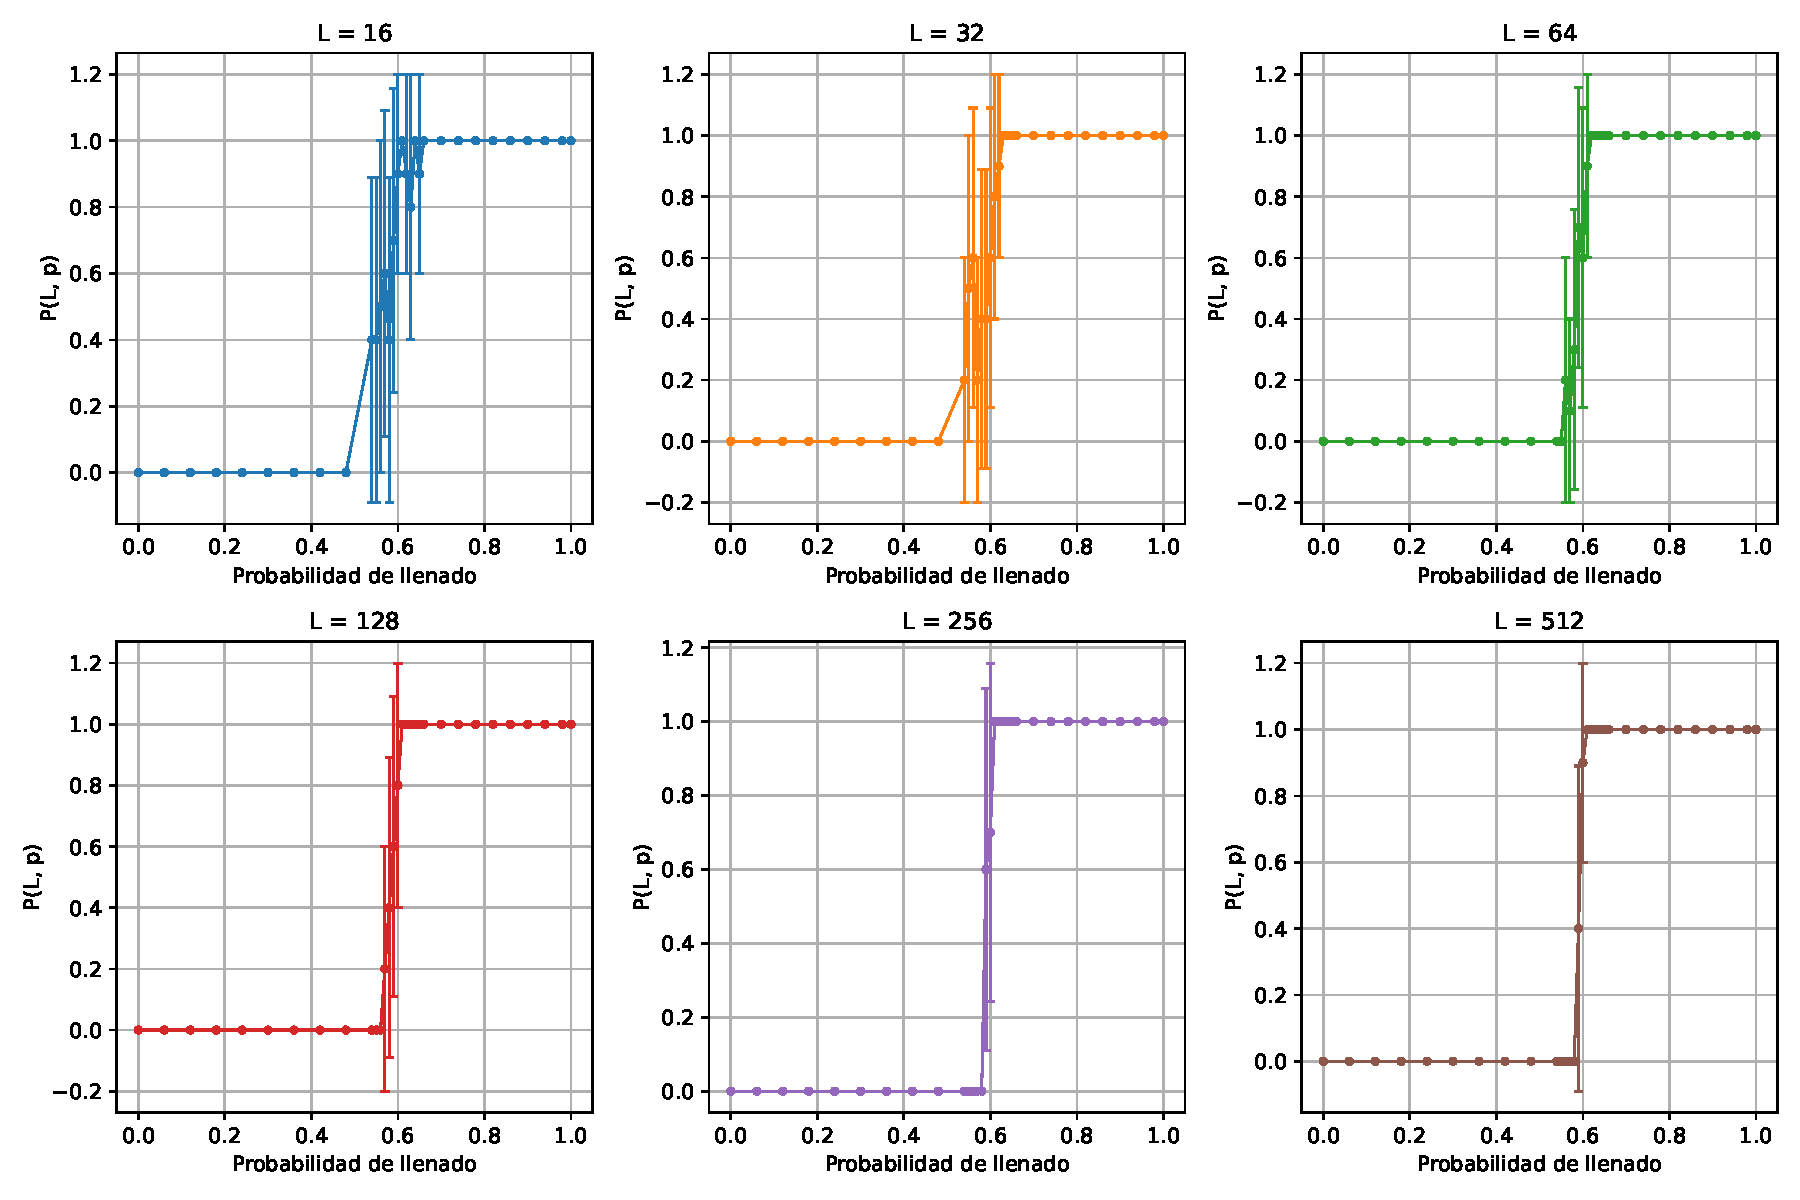
\includegraphics[width=1.0\textwidth]{figures/Perc_prob.pdf}
    \caption{Probabilidad de percolación \(P(L,p)\) frente a la probabilidad de llenado \(p\), para redes cuadradas de tamaño \(L = 16,\,32,\,64,\,128,\,256,\,512\). Se observa una transición en la probabilidad de percolación que se hace más pronunciada al aumentar \(L\).}
    \label{fig:perc_prob}
\end{figure}

Por otro lado, en la Figura \ref{fig:size} se grafica el tamaño promedio del clúster percolante más grande normalizado en función de \(p\). No hay casi datos para \(p\) por debajo del umbral crítico \(p_c\) dado que en estos casos es muy poco probable que se presente percolación (no hay clúster macroscópico). Para los valores de \(p\) tomados en cuenta, se observa un crecimiento pronunciado cerca de \(p_c\) y posteriormente un crecimiento lineal de \(S(L,p)\) hasta llegar al tamaño del sistema con \(p = 1\) como es esperado. Igualmente, el punto de inflexión en donde comienza un crecimiento lineal se da aproximadamente para un tamaño de aproximadamente el 60\% del sistema para todos los valores de L. Sin embargo, conforme \(L\) crece la varianza en los datos disminuye y se obtiene una curva suave, acercandose al caso ideal del limite termodinámico.

\begin{figure}[ht]
    \centering
    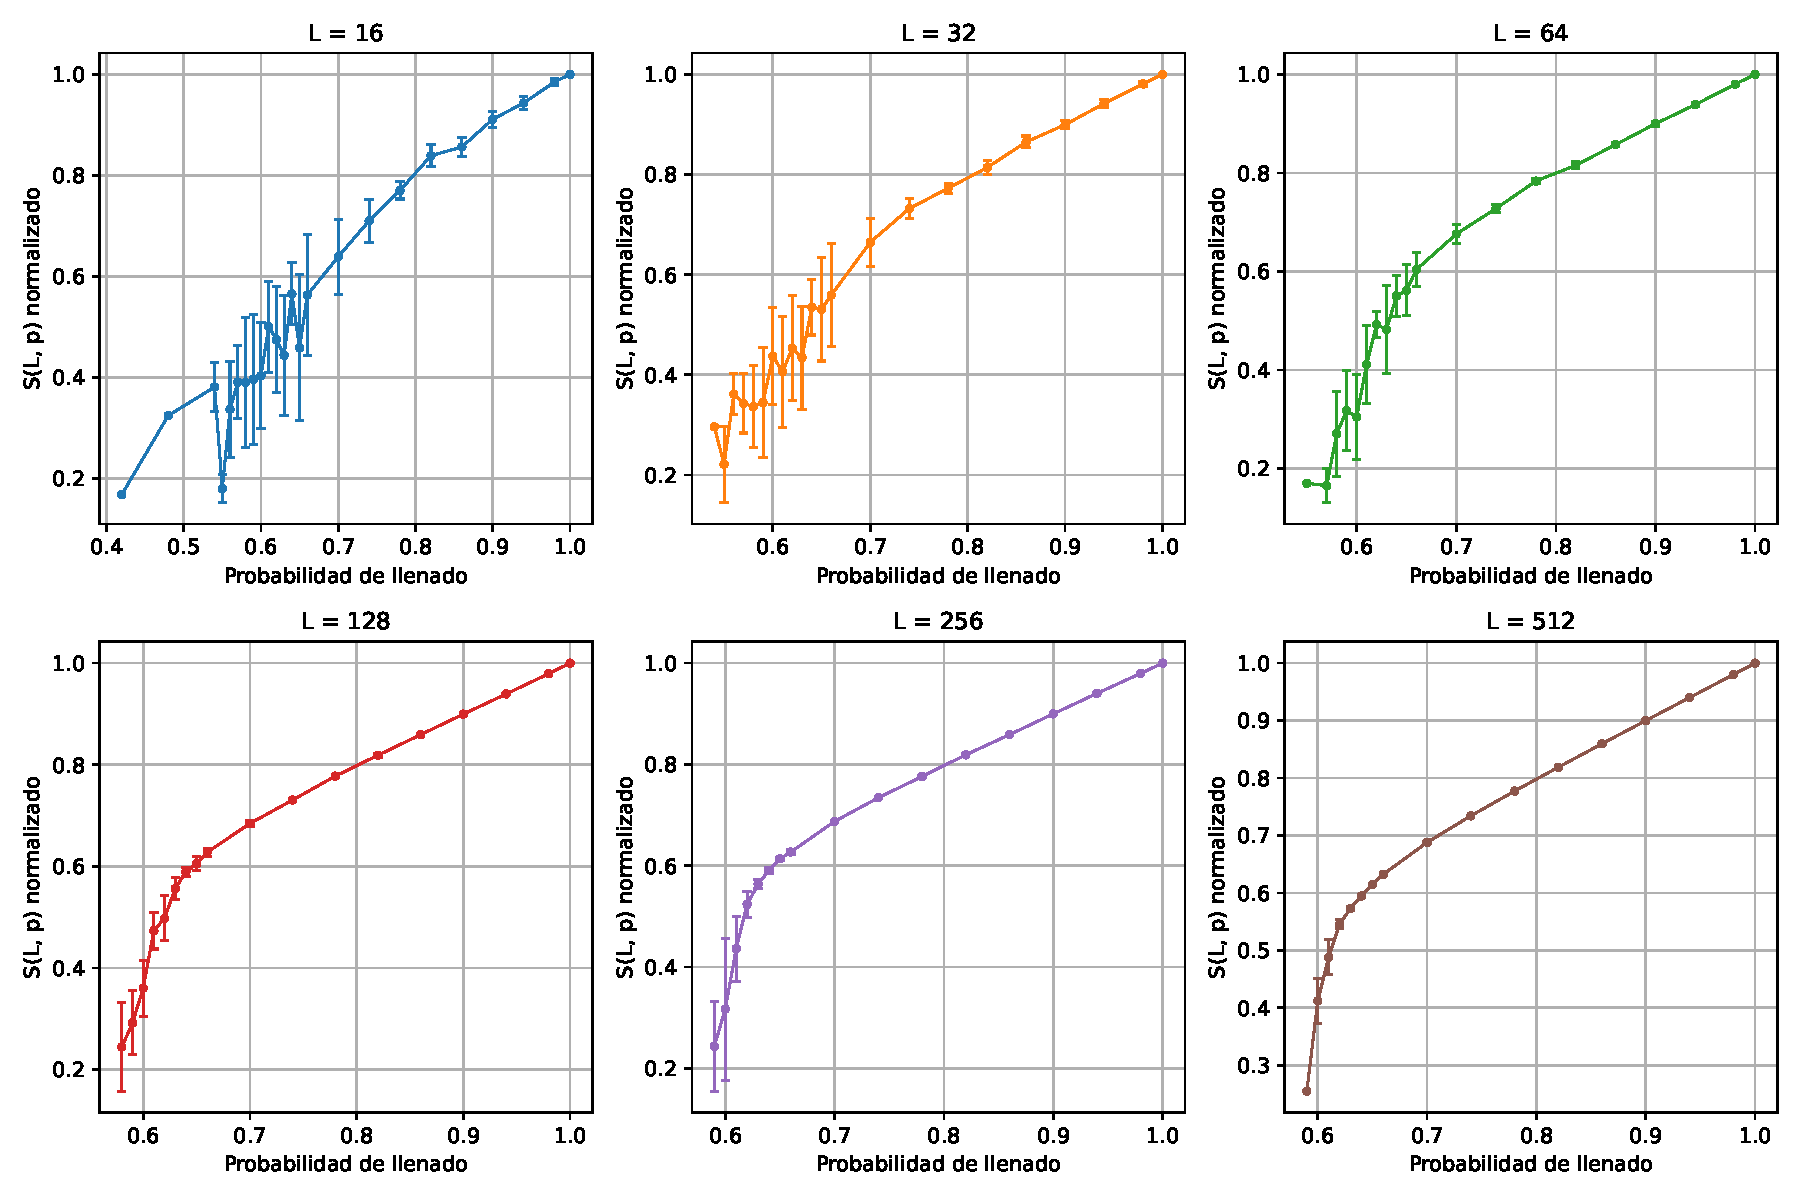
\includegraphics[width=1.0\textwidth]{figures/Size.pdf}
    \caption{Tamaño promedio del clúster percolante más grande normalizado, \(S(L,p) = ( \text{tamaño del clúster mayor} ) / L^2\), frente a la probabilidad de llenado \(p\), para redes cuadradas de tamaño \(L = 16,\,32,\,64,\,128,\,256,\,512\). Se aprecia el crecimiento pronunciado de \(S\) alrededor del umbral crítico.}
    \label{fig:size}
\end{figure}

\section{Análisis profiling}

\subsection{Niveles de optimización}
Para evaluar el impacto de los distintos niveles de optimización del compilador en el rendimiento de nuestro programa de percolación, compilamos el código con las banderas \texttt{-O0}, \texttt{-O1}, \texttt{-O2}, \texttt{-O3} y \texttt{-Ofast}. A continuación, la Figura~\ref{fig:opt_levels} muestra el tiempo de ejecución medido (en milisegundos) para diferentes tamaños de red \(L\) y la probabilidad de llenado \(p = 0.6\) cercana a la probabilidad crítica.

\begin{figure}[h!]
    \centering
    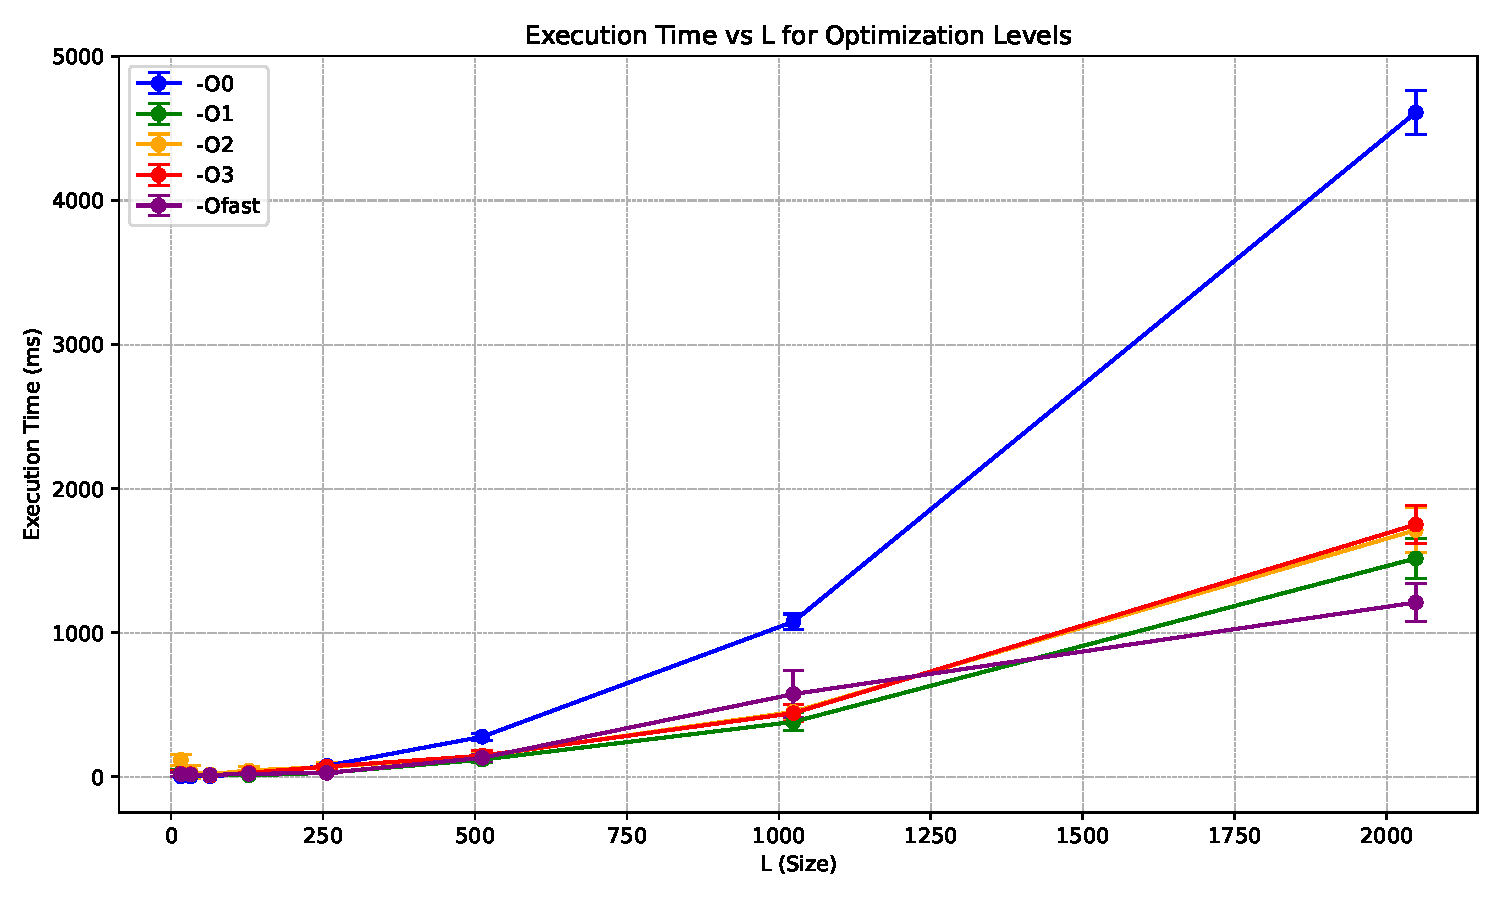
\includegraphics[width=1.0\textwidth]{figures/opti_comparison.pdf}
    \caption{Tiempo de ejecución del programa de percolación en función del tamaño de la red \(L\), compilado con distintos niveles de optimización: \texttt{-O0} (sin optimizar), \texttt{-O1}, \texttt{-O2}, \texttt{-O3} y \texttt{-Ofast}.}
    \label{fig:opt_levels}
\end{figure}

En general, se observa que el tiempo de ejecución es muy corto incluso para un tamaño del sistema \(L \approx 2000\) y una optimización \texttt{-O0}. Además, el tiempo de ejecución disminuye significativamente al aplicar optimizaciones, siendo \texttt{-O3} y \texttt{-Ofast} las más efectivas, reduciendo el tiempo de ejecución a menos de 1 segundo para \(L = 2000\). La optimización \texttt{-Ofast} es la más rápida, pero puede introducir cambios en el comportamiento del programa al desactivar ciertas verificaciones de precisión. Por otro lado, la optimización \textit{-O0} muestra un rendimiento significativamente peor, lo que indica que las optimizaciones del compilador son cruciales para mejorar la eficiencia del código, especialmente en algoritmos que requieren múltiples iteraciones y operaciones sobre estructuras de datos como matrices y vectores. Vemos también que, para tamaños pequeños, la diferencia entre los niveles de optimización es imperceptible, pero a medida que \(L\) aumenta, las optimizaciones tienen un impacto más significativo en el tiempo de ejecución.

\subsection{Informe profiling}
Se realizó un informe detallado de \textit{profiling} utilizando \texttt{gprof}. Sin embargo, debido al uso de librerías sobre las cuales no se tiene control, resultaba difícil obtener información precisa sobre el comportamiento interno del programa. Por esta razón, se filtró el reporte para mostrar únicamente las funciones definidas explícitamente en el código del proyecto. Este informe filtrado se incluye en el Anexo~\ref{app:flat_profile}. Como se puede observar, las funciones creadas corresponden a menos del 10\% del tiempo total de ejecución. Por lo tanto, se concluye que el algoritmo implementado es sumamente eficiente y que la mayor parte del tiempo se consume en llamadas a funciones de la biblioteca estándar de \texttt{C++}.

Adicionalmente, se generó un reporte plano con \texttt{perf}, el cual proporciona información complementaria y una mayor resolución temporal en comparación con \texttt{gprof}. A partir de este reporte, se generó un \textit{flamegraph} que permite visualizar jerárquicamente las llamadas a funciones y el tiempo acumulado en cada una. En la Figura~\ref{fig:flamegraph} se presenta dicho \textit{flamegraph}, donde el largo de cada banda corresponde al tiempo de CPU consumido por esa función y sus subllamadas. Esta herramienta resulta particularmente útil para identificar visualmente los puntos más costosos en términos de tiempo de ejecución. El reporte plano usado como base se incluye en el Anexo~\ref{app:flat_profile_perf}.

\begin{figure}[h!]
    \centering
    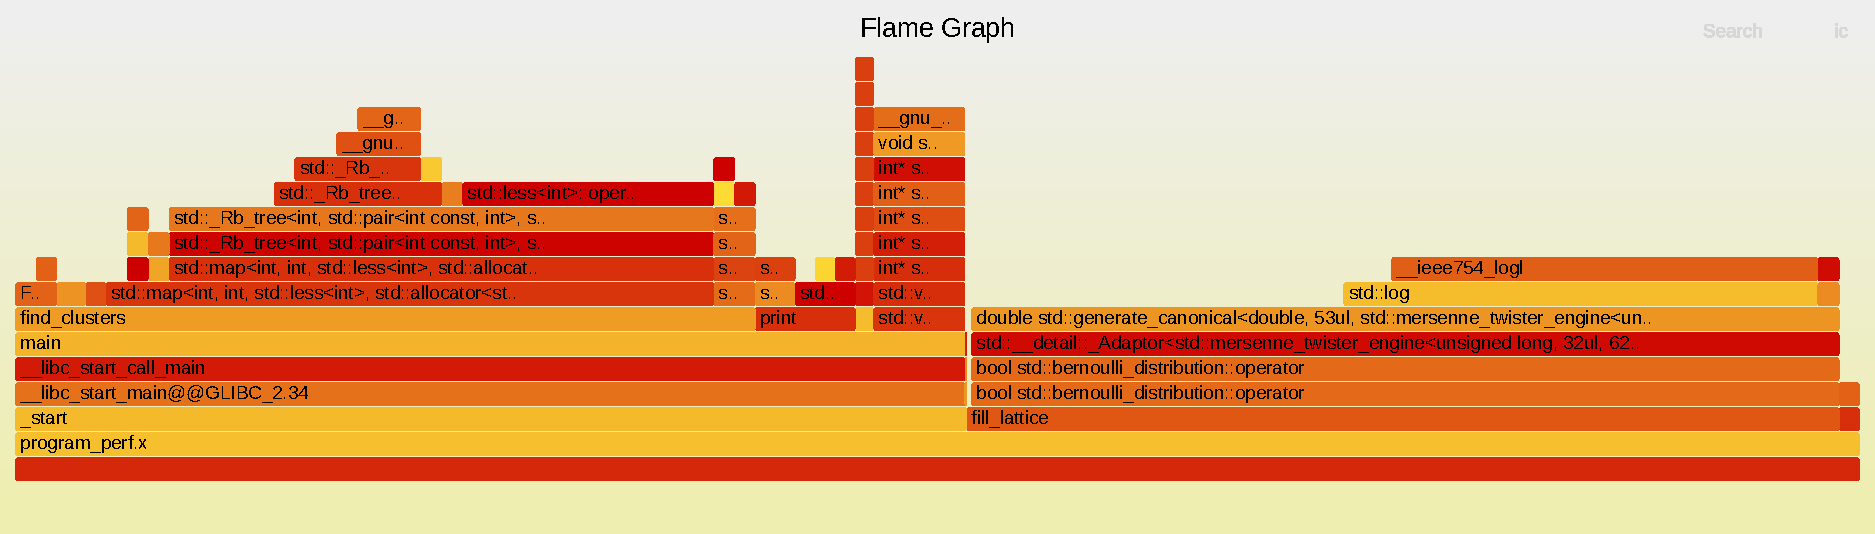
\includegraphics[width=1.0\textwidth]{figures/flamegraph.pdf}
    \caption{Flamegraph del perfil de ejecución generado con \texttt{perf}.}
    \label{fig:flamegraph}
\end{figure}

Como se observa en la Figura~\ref{fig:flamegraph}, las funciones que concentran el mayor uso de CPU son \texttt{find\_clusters} y \texttt{print}, seguidas por \texttt{HoshenKopelman} y \texttt{fill\_lattice}. La función \texttt{find\_clusters} es responsable de identificar los clústeres en la red, mientras que \texttt{print} se encarga de mostrar los resultados. Por otro lado, \texttt{HoshenKopelman} es el algoritmo que etiqueta los clústeres y \texttt{fill\_lattice} llena la red con ocupación aleatoria. Estas funciones son críticas para el rendimiento del programa, ya que representan las operaciones más costosas en términos de tiempo de ejecución. No obstante, y como ya mencionó anteriormente, al analizar los reportes planos de \texttt{perf} y \texttt{gprof}, se evidencia que gran parte del tiempo dentro de estas funciones se consume en llamadas a funciones de la biblioteca estándar, como operaciones de inserción y recorrido de estructuras \texttt{std::map} o el uso de \texttt{std::ostream}, lo cual sugiere que las estructuras y métodos utilizados internamente también tienen un impacto significativo en el rendimiento general del programa, lo que limita las oportunidades de optimización a nivel de código fuente.



\section{Optimizaciones realizadas}

El análisis del reporte de profiling mostró que las funciones definidas en nuestro código consumen un porcentaje muy bajo del tiempo total, por lo que no se identificaron optimizaciones significativas a través de gprof. Sin embargo, al examinar las gráficas de tiempos de ejecución con distintos niveles de compilación y revisar detenidamente el código, detectamos algunas mejoras puntuales: en lugar de inicializar el vector de etiquetas con un tamaño fijo de \(L^2/2\) y llenarlo, resultó más eficiente usar \texttt{$labels.push_back()$} dado que el número real de etiquetas es generalmente mucho menor que \(L^2/2\). Asimismo, la obtención de \texttt{$unique_ids$} se cambió de operar sobre la matriz completa a utilizar directamente el vector \texttt{labels}, más pequeño y suficiente para nuestro propósito. Finalmente, en la función de \texttt{Find} se implementó la rutina de compresión de camino, permitiendo que en llamadas porteriores se encontrara el cluster padre un poco más rapido, esto es especialmente util dado que es la función que más veces se llama en el codigo cómo lo demuestra el reporte de\texttt{gprof} . El código mencionado se observa en el Listing \ref{lst:opt_codigo_sin_acentos}. 
 
\begin{lstlisting}[language=C++,caption={Codigo de optimizaciones}, label={lst:opt_codigo_sin_acentos}]
    // ------------ Funcion HoshenKopelman: ------------
    //   Inserta nueva etiqueta en el vector de labels
    labels.push_back(next_label);
    
    // ------------ Funcion find_clusters: ------------
    //   Crea un unique_ids con vec labels en lugar de lattice 
    std::set<int> unique_ids(labels.begin(), labels.end()); 

    // ------------ Funcion Find: ------------
    //   Compresion de camino en union-find
    while (parent[ii] != ii) {
        kk = parent[ii];
        parent[ii] = jj;
        ii = kk;
    }
\end{lstlisting}


\section{Conclusiones}
El proyecto de percolación ha permitido explorar y comprender el fenómeno de percolación en redes bidimensionales, implementando el algoritmo de Hoshen-Kopelman para identificar clústeres y determinar la probabilidad de percolación. Los resultados obtenidos muestran una transición clara en la probabilidad de percolación a medida que se varía la probabilidad de llenado \(p\), corroborando las predicciones teóricas del modelo.
Además, se ha realizado un análisis exhaustivo del rendimiento del código mediante herramientas de profiling como \texttt{gprof} y \texttt{perf}, lo que ha permitido identificar las funciones más críticas en términos de tiempo de ejecución. Aunque el código original ya era eficiente, se implementaron algunas optimizaciones menores que mejoraron ligeramente el rendimiento, especialmente en la gestión de estructuras de datos.
El uso de distintos niveles de optimización del compilador ha demostrado ser crucial para mejorar el rendimiento del programa, especialmente en tamaños de red grandes. Las optimizaciones más agresivas (\texttt{-O3} y \texttt{-Ofast}) lograron reducir significativamente el tiempo de ejecución, aunque con un pequeño riesgo de alterar el comportamiento del programa.
Finalmente, se observó que gran parte del tiempo de CPU se concentra en operaciones internas de funciones estándar de C++, como manejo de mapas y flujo de salida, más que en la lógica explícita del algoritmo implementado.


\clearpage
\appendix
\section{Anexos}

\subsection{Flat profile de \texttt{gprof} filtrado}
\label{app:flat_profile}

A continuación se presenta el perfil plano (flat profile) generado por \texttt{gprof}, filtrado para mostrar únicamente las funciones definidas en el código del proyecto (se han eliminado entradas de librerías del sistema).

\lstinputlisting[caption={Flat profile filtrado de gprof},label={lst:gprof_filtered}]{out_report/report_gprof_filtered.txt}

\subsection{Flat profile de \texttt{perf} filtrado}
\label{app:flat_profile_perf}

A continuación se presenta el perfil plano (flat profile) generado por \texttt{perf}, filtrado para mostrar únicamente las funciones definidas en el código del proyecto (se han eliminado entradas de librerías del sistema).

\lstinputlisting[caption={Flat profile filtrado de perf},label={lst:perf_filtered}]{out_report/report_perf_filtered.txt}

\end{document}
